\documentclass[10pt]{article}
\usepackage{amsmath}
\usepackage[hidelinks]{hyperref}
\usepackage{amssymb}
\usepackage{tikz}
\usepackage{caption}
\usepackage{graphicx}
\graphicspath{{.}}
\usepackage{listings}
\usepackage{verbatim}
\lstset{
language=[LaTeX]TeX,
backgroundcolor=\color{gray!25},
basicstyle=\ttfamily,
columns=flexible,
breaklines=true
}
\captionsetup{labelsep=space,justification=justified,singlelinecheck=off}
\reversemarginpar
\usepackage[paper=a4paper,
            %includefoot, % Uncomment to put page number above margin
            marginparwidth=20mm,      % Length of section titles
            marginparsep=0.8mm,       % Space between titles and text
            margin=12mm,              % 25mm margins
            includemp]{geometry}

\begin{document}
\section*{}
\begin{flushleft}
CSCI 5502 - Data Mining - Homework 2\\
Name: Krishna Chaitanya Sripada\\
Student ID: 104375417\\
Honor Pledge: On my honor, as a University of Colorado at Boulder student, I have neither given nor received unauthorized assistance on this work.
\end{flushleft}
\section*{Ans 1.}
\begin{flushleft}
Code has been submitted
\end{flushleft}
\section*{Ans 2.}
\begin{flushleft}
a. A single plot showing the temporal change of the ``High'' and ``Low'' attributes:\\
\begin{figure}[!htb]
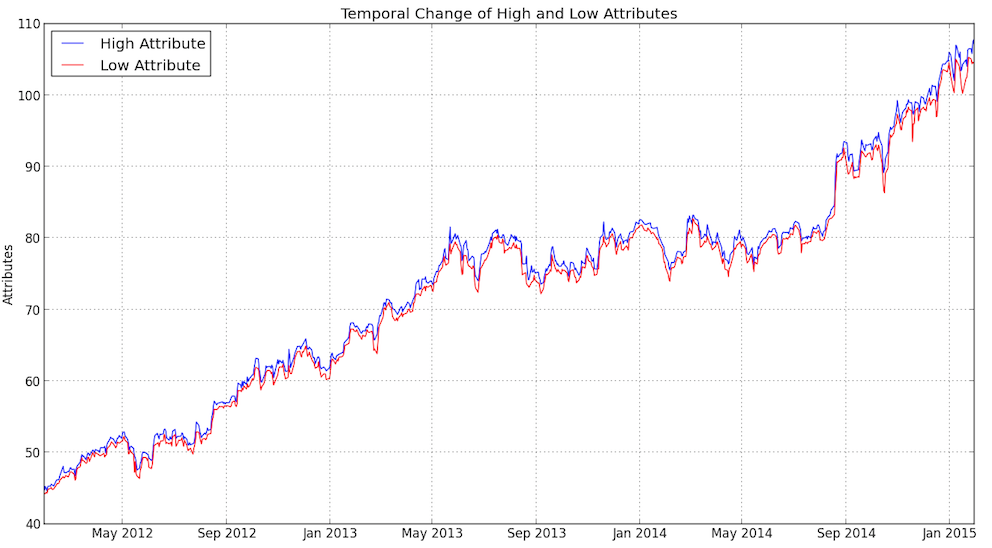
\includegraphics{Plot-1_1}
\caption{:Temporal change of the ``High'' and ``Low'' attributes}   
\label{fig::Temporal change of the ``High'' and ``Low'' attributes} 
\end{figure}
\vspace{30em}
b. A boxplot for the ``Open'' and ``Close/Last'' attributes.\\
\begin{figure}[!htb]
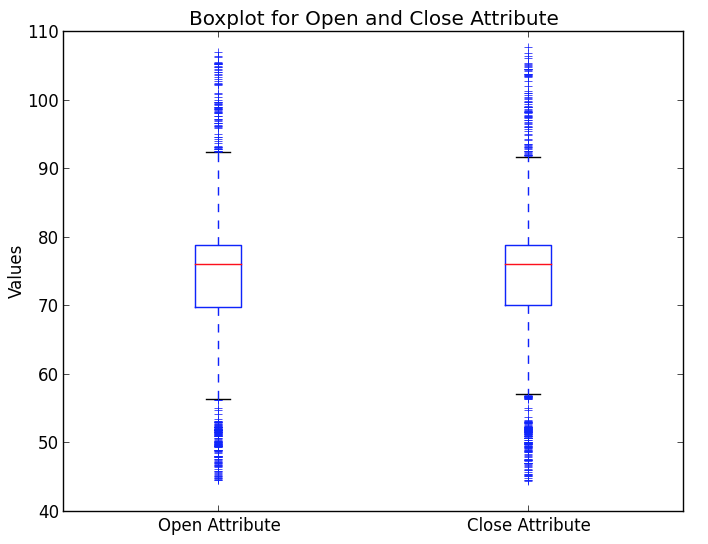
\includegraphics{Plot-2_1}
\caption{:A boxplot for the ``Open'' and ``Close/Last'' attributes}   
\label{fig::A boxplot for the ``Open'' and ``Close/Last'' attributes} 
\end{figure}
c. The 10-bin equal-width histogram for the ``Volume'' attribute.\\
\begin{figure}[!htb]
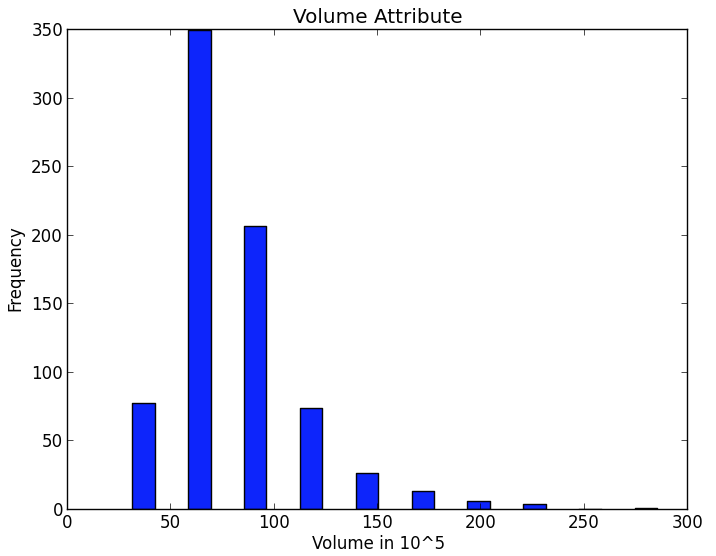
\includegraphics{Plot-3_1}
\caption{:The 10-bin equal-width histogram for the ``Volume'' attribute}   
\label{fig::The 10-bin equal-width histogram for the ``Volume'' attribute} 
\end{figure}
\vspace{30em}
d. Quantile Probability plot for ``Open'' Attribute.\\
\begin{figure}[!htb]
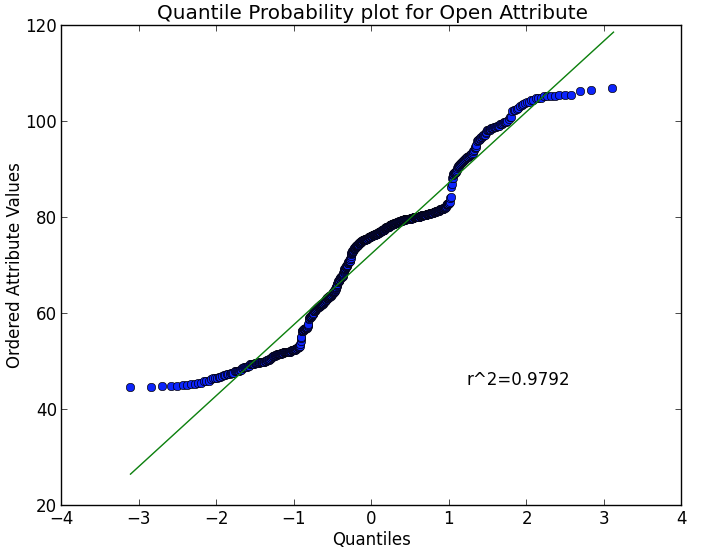
\includegraphics{Plot-4_1}
\caption{:Quantile Probability plot for ``Open'' Attribute}   
\label{fig::Quantile Probability plot for ``Open'' Attribute} 
\end{figure}
\end{flushleft}
\end{document}